\documentclass[12pt]{article}
\usepackage[english]{babel}
\usepackage{natbib}
\usepackage{url}
\usepackage[utf8x]{inputenc}
\usepackage{amsmath}
\usepackage{graphicx}
\graphicspath{{Images/}}
\usepackage{parskip}
\usepackage{fancyhdr}
\usepackage{vmargin}
\setmarginsrb{3 cm}{2.5 cm}{3 cm}{2.5 cm}{1 cm}{1.5 cm}{1 cm}{1.5 cm}

\title{Introducción a Python, Jupyter y Pandas}								% Title
\author{Martha Anahí Iñiguez Beltrán}						% Author
\date{\today}											% Date

\makeatletter
\let\thetitle\@title
\let\theauthor\@author
\let\thedate\@date
\makeatother

\pagestyle{fancy}
\fancyhf{}
\rhead{Física Computacional}
\lhead{\thetitle}
\cfoot{\thepage}

\begin{document}

\begin{titlepage}
\centering
    \vspace*{0.5 cm}

    \textsc{\LARGE Universidad de Sonora}\\[2.0 cm]	% University Name
    \textsc{\Large Departamento de ciencias exactas}\\[1.0 cm]
\textsc{\Large Física Computacional}\\[0.5 cm]
\rule{\linewidth}{0.2 mm} \\[0.4 cm]
{ \huge \bfseries \thetitle}\\
\rule{\linewidth}{0.2 mm} \\[1.5 cm]
\begin{minipage}{0.6\textwidth}
\begin{flushleft} \large
\emph{Alumno:}\\
\theauthor
\end{flushleft}
\end{minipage}~
\begin{minipage}{0.4\textwidth}
\begin{flushright} \large
214202804
\end{flushright}
\end{minipage}\\[2 cm]


{\large \thedate}\\[2 cm]

\vfill

\end{titlepage}

\tableofcontents
\pagebreak


\section{Introducción}
\noindent

En la siguiente actividad aprenderemos y prácticaremos el uso del lenguaje de programación Python, iniciando con comandos simples y hasta el desarrollo de tablas y gráficas basadas en bases de datos previamente elaboradas y revisadas.

Todo lo anterior se realizara por medio de la aplicación web "Jupyter Notebook".

\begin{centering}
\centering
\begin{figure}
  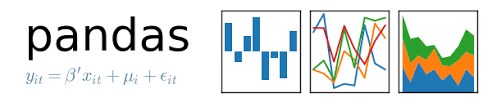
\includegraphics[scale = 0.4]{descarga.png}
\end{figure}
\end{centering}

\section{Jupyter}

Jupyter notebook es una aplicación web que permite crear, editar y compartir documentos que contengan código, ecuaciones, visualizaciones y texto explicativo.

Algunas de sus características principales son:

- Texto marcado (con cabeceros, estilos, parrafos, etc).\\- Fórmulas, matematicas, gráficos, mapas, etc\\- Bibliotecas externas importadas para añadir funcionalidades.\\- Código de múltiples lenguajes de programación, incluyendo python, R, Julia, Bash y muchos más.

Su uso incluye la limpieza y transformación de memoria, simulación numérica, modelos estadísticos, entre otras funciones.

\subsection{Beneficios de Jupyter}

Uno de los más importantes beneficios de Jupyter es que soporta alrededor de 40 distintos lenguajes de programación. Entre ellos están:

- Python\\- R\\- Julia\\- Scala\\- Fortran\\- MATLAB\\- Babel\\- Java 9

Podemos manejarlo desde la terminal y utilizar bases de datos e imágenes  previamente almacenadas en la misma carpeta donde iniciamos el Kernel.

\section{Actividad}

Para comenzar con el manejo de Python, Jupyter y Pandas generamos el siguiente código, el cual fue un análisis de datos obtenidos por el Servicio Meteorológico Nacional y del cual obtuvimos datos como la velocidad de los vientos y ráfagas, la temperatura, la radiación solar, etc.

Los datos anteriormente mencionados fueron obtenidos por la estación de recopilación de datos automática "Cumbre de mty 1", ubicada en Monterrey, Nuevo León.

El código es el siguiente.

\subsection{Código de la Actividad 2}
\begin{verbatim}

# Cargar a la memoria de trabajo las bibliotecas: Pandas (manejo de datos, 
# Numpy (numerical python) y la biblioteca de gráficas Matplotlib
# Se asignan nombres cortos.
import pandas as pd
import numpy as np
import matplotlib.pyplot as plt
#
# Usar "Shift+Enter" para procesar la información de la celda
#

# Descarga los datos de una estación del Servicio Meteorológico Nacional
# http://smn1.conagua.gob.mx/emas/
# Lee un archivo de texto con la función Pandas "read_csv", con elementos
#separados por mas de 
# un espacio, brincándose 4 renglones del inicio (encabezados)
df0 = pd.read_csv('monterrey.txt', skiprows=4, sep='\s+')

# Lee los primeros 5 renglones del archivo
df0.head()

# Dar estructura de datos (DataFrame)
df = pd.DataFrame(df0)

# Combinar las columnas "DD/MM/AAAA" con "HH:MM" y convertirla a variable de 
#tiempo
# Se crea una nueva columna "Fecha" al final con formato de tiempo.
# Eliminamos las dos primeras columnas que ya no necesitaremos
df['FECHA'] = pd.to_datetime(df.apply(lambda x: x['DD/MM/AAAA'] + ' ' + x['HH:MM'], 1), dayfirst=True)
df = df.drop(['DD/MM/AAAA', 'HH:MM'], 1)

df.head()

# Realiza un análisis exploratorio de datos
df.describe()

# Selecciona los renglones con Temperatura > 24ºC y < 25ºC
df_tmp = df[df.TEMP > 24] 
df_select = df_tmp[df_tmp.TEMP < 25]
df_select

# Calcula el promedio de las columnas, excepto en la FECHA (que no tendría
#sentido)
df.mean()

# Calcula el promedio de las Temperaturas
df.TEMP.mean()

# Gráfica de la rapidez de los vientos (m/s) 
plt.figure(); df.VELS.plot(); plt.legend(loc='best')
plt.title("Variación de la Rapidez de los Vientos")
plt.ylabel("Rapidez (m/s)")
plt.grid(True)
plt.show()

# Gráfica de Temperatura y Humedad Relativa
df1 = df[['TEMP','HR']]
plt.figure(); df1.plot(); plt.legend(loc='best')
plt.title("Variación de la Temperatura y la Humedad Relativa")
plt.ylabel("Temp ºC /(%) HR")
plt.grid(True)
plt.show()

#Comentario acerca de la temperatura y la humedad relativa
Siguiendo los datos que nos proporciona la gráfica podemos notar que entre 
más alta es la temperatura, más baja será la humedad relativa. Siguiendo esto, concluímos que cuando la temperatura baja, la humedad relativa aumenta.

plt.plot_date(x=df.FECHA, y=df.TEMP, fmt="b-")
plt.title("Variación de la Temperatura")
plt.ylabel("Temp ºC")
plt.grid(True)
plt.show()

# Gráfica de Rapidez de los vientos y Rapidez de las ráfagas
df1 = df[['VELS','VELR']]
plt.plot_date(x=df.FECHA, y=df1, fmt='-')
plt.title("Rapidez de vientos y rafagas como funciones del tiempo")
plt.ylabel("Rapidez (Km/h)")
plt.xlabel("Fecha")
plt.grid(True)
plt.show()

# Gráfica de Direccion de los vientos y Direccion de las ráfagas
df1 = df[['DIRS','DIRR']]
plt.plot_date(x=df.FECHA, y=df1, fmt='-')
plt.title("Direccion de vientos y rafagas como funciones del tiempo")
plt.ylabel("Direccion (Grados)")
plt.xlabel("Fecha")
plt.grid(True)
plt.show()

#Entrada como Markdown
Analizando la gráfica podemos notar que los vientos dominantes son los que rondan
los 100 a 250 grados.

#Gráfica de la radiación solar en función del tiempo
plt.plot_date(x=df.FECHA, y=df.RADSOL, fmt="c-")
plt.title("Variación de la Radiación Solar")
plt.ylabel("Radiación solar (W/m2)")
plt.xlabel("Fecha")
plt.grid(True)
plt.show()

#Comentario acerca de la radiación solar
Dependiendo de la hora del día se puede detectar mayor o menor emisión de 
radiación solar.

#Análisis exploratorio de datos sobre el dataframe
df.describe()

\end{verbatim}

\section{Resultados}

Como resultado de la actividad podemos incluir las gráficas obtenidas por el programa las cuales son las siguientes.

\begin{figure}
\begin{centering}
  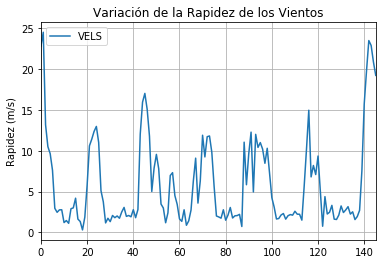
\includegraphics[scale = 0.8]{VarRapVie.png}
  \caption{Gráfica de la rapidez de los vientos}
\end{centering}
\end{figure}

\begin{figure}
\begin{centering}
  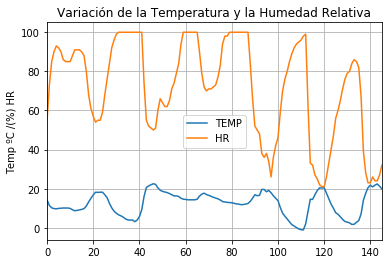
\includegraphics[scale = 0.8]{vaTH.png}
  \caption{Gráfica de temperatura y humedad relativa}
\end{centering}
\end{figure}

\begin{figure}
\begin{centering}
  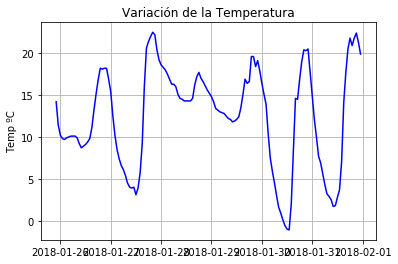
\includegraphics[scale = 0.8]{vaT.png}
  \caption{Gráfica de fecha y temperatura}
\end{centering}
\end{figure}

\begin{figure}
\begin{centering}
  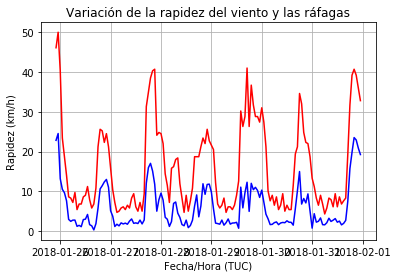
\includegraphics[scale = 0.8]{VieRaf.png}
  \caption{Gráfica de la rapidez de las ráfagas}
\end{centering}
\end{figure}

\begin{figure}
\begin{centering}
  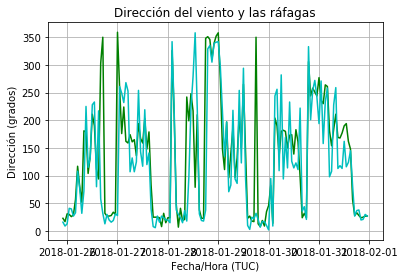
\includegraphics[scale = 0.8]{dirVieRaf.png}
  \caption{Gráfica de la dirección de los vientos}
\end{centering}
\end{figure}

\begin{figure}
\begin{centering}
  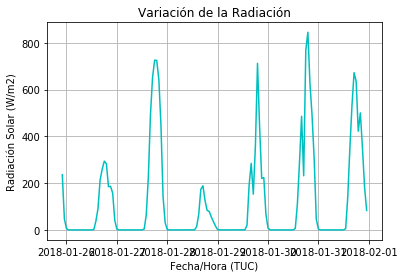
\includegraphics[scale = 0.8]{varRadSol.png}
  \caption{Gráfica de la radiación solar}
\end{centering}
\end{figure}

\section{Apéndice}

En esta sección responderemos preguntas respecto a la actividad realizada.

\textbf{¿Cuál es tu primera impresión de Jupyter Notebook?}

\textbf{¿Se te dificultó leer código en Python?}

Fue algo nuevo pero no difícil, es más claro leer el código a comparación de otros lenguajes ya que, en conjunto con jupyter, va saliendo lo que le estamos pidiendo que haga.

\textbf{¿En base a tu experiencia de programación en Fortran, que te parece el entorno de trabajar en Python?}

Es un poco más sencillo pues se está compilando al mismo tiempo que se avanza con el código y podemos notar desde un principio si hay alguna falla para abordarla antes de seguir con el prográma.

\textbf{A diferencia de Fortran, ahora se producen las gráficas utilizando la biblioteca Matplotlib. ¿Cómo fue tu experiencia?. }

Me parece más sencillo la manera en que se producen las gráficas y son más atractivas visualmente, sin embargo, preferiría poder cambiar el tamaño.

\textbf{En general, ¿qué te pereció el entorno de trabajo en Python? }

Me parece bueno, es más sencillo, ordenado y completo.

\textbf{¿Qué opinas de la actividad? ¿Estuvo compleja? ¿Mucho material nuevo? ¿Que le faltó o que le sobró? ¿Qué modificarías para mejorar? }

Personalmente no tenía mucho conocimiento de cómo programar con Python y me pareció una actividad sencilla y nueva. Me brindó material nuevo para trabajar con futuras actividades. Me hubiera gustado ver como introducir ecuaciones a partir de la base de datos que manejamos.

\textbf{¿Comentarios adicionales que desees compartir? }

La actividad estuvo completa, salvo el comentario en la respuesta anterior. Sin embargo hay mucho material nuevo para utilizar.

\end{document}

%configuration={"latex_command":"latexmk -pdf -f -g -bibtex -synctex=1 -interaction=nonstopmode 'Actividad2-práctica1.tex'"}
